% Options for packages loaded elsewhere
\PassOptionsToPackage{unicode}{hyperref}
\PassOptionsToPackage{hyphens}{url}
%
\documentclass[
  10pt,
  a4paper,
]{article}
\usepackage{amsmath,amssymb}
\usepackage{iftex}
\ifPDFTeX
  \usepackage[T1]{fontenc}
  \usepackage[utf8]{inputenc}
  \usepackage{textcomp} % provide euro and other symbols
\else % if luatex or xetex
  \usepackage{unicode-math} % this also loads fontspec
  \defaultfontfeatures{Scale=MatchLowercase}
  \defaultfontfeatures[\rmfamily]{Ligatures=TeX,Scale=1}
\fi
\usepackage{lmodern}
\ifPDFTeX\else
  % xetex/luatex font selection
\fi
% Use upquote if available, for straight quotes in verbatim environments
\IfFileExists{upquote.sty}{\usepackage{upquote}}{}
\IfFileExists{microtype.sty}{% use microtype if available
  \usepackage[]{microtype}
  \UseMicrotypeSet[protrusion]{basicmath} % disable protrusion for tt fonts
}{}
\makeatletter
\@ifundefined{KOMAClassName}{% if non-KOMA class
  \IfFileExists{parskip.sty}{%
    \usepackage{parskip}
  }{% else
    \setlength{\parindent}{0pt}
    \setlength{\parskip}{6pt plus 2pt minus 1pt}}
}{% if KOMA class
  \KOMAoptions{parskip=half}}
\makeatother
\usepackage{xcolor}
\usepackage[margin=20mm]{geometry}
\usepackage{longtable,booktabs,array}
\usepackage{calc} % for calculating minipage widths
% Correct order of tables after \paragraph or \subparagraph
\usepackage{etoolbox}
\makeatletter
\patchcmd\longtable{\par}{\if@noskipsec\mbox{}\fi\par}{}{}
\makeatother
% Allow footnotes in longtable head/foot
\IfFileExists{footnotehyper.sty}{\usepackage{footnotehyper}}{\usepackage{footnote}}
\makesavenoteenv{longtable}
\usepackage{graphicx}
\makeatletter
\def\maxwidth{\ifdim\Gin@nat@width>\linewidth\linewidth\else\Gin@nat@width\fi}
\def\maxheight{\ifdim\Gin@nat@height>\textheight\textheight\else\Gin@nat@height\fi}
\makeatother
% Scale images if necessary, so that they will not overflow the page
% margins by default, and it is still possible to overwrite the defaults
% using explicit options in \includegraphics[width, height, ...]{}
\setkeys{Gin}{width=\maxwidth,height=\maxheight,keepaspectratio}
% Set default figure placement to htbp
\makeatletter
\def\fps@figure{htbp}
\makeatother
\setlength{\emergencystretch}{3em} % prevent overfull lines
\providecommand{\tightlist}{%
  \setlength{\itemsep}{0pt}\setlength{\parskip}{0pt}}
\setcounter{secnumdepth}{-\maxdimen} % remove section numbering
\usepackage{float}
\usepackage{fancyhdr}
\pagestyle{fancy}\fancyhf{}
\fancyhead[L]{\small FMAT3888: Portfolio Construction}
\fancyhead[R]{\small Question 2(a)--(d)}
\fancyfoot[C]{\thepage}
\setlength{\headheight}{14pt}
\setlength{\parskip}{5pt}
\ifLuaTeX
  \usepackage{selnolig}  % disable illegal ligatures
\fi
\IfFileExists{bookmark.sty}{\usepackage{bookmark}}{\usepackage{hyperref}}
\IfFileExists{xurl.sty}{\usepackage{xurl}}{} % add URL line breaks if available
\urlstyle{same}
\hypersetup{
  hidelinks,
  pdfcreator={LaTeX via pandoc}}

\author{}
\date{}

\begin{document}

\hypertarget{question-2-static-portfolio-optimisation}{%
\section{Question 2: Static Portfolio
Optimisation}\label{question-2-static-portfolio-optimisation}}

\hypertarget{overview-and-inputs}{%
\subsection{Overview and inputs}\label{overview-and-inputs}}

We use the expected-return vector m and covariance matrix C from Q1 to
construct portfolios, subject to full investment, no short selling and a
50\% limit on each index. The uncapped long-only portfolio is used as a
benchmark for comparison of different index caps; 40\% and 30\% caps and
unrestricted signed weights are alternative comparisons.

The analysis answers all four parts of Q2: constraints and
efficient-frontier plots; the global minimum-variance portfolio;
portfolios for a range of return requirements; and sensitivity to
alternative Q1 estimates.

Q1 provides 248 simple monthly returns from 31 January 2006 to 31 August
2026, calculated from 249 common monthly index levels. Each index uses
the same dates. We retain Q1's annualisation: m equals 12 times the
average monthly return, and C equals 12 times the sample monthly
covariance matrix, using denominator N - 1. These are annualised
arithmetic estimates, not compound annual growth rates.

\begin{longtable}[]{@{}lrr@{}}
\toprule\noalign{}
Index & Annualised expected return & Annualised volatility \\
\midrule\noalign{}
\endhead
\bottomrule\noalign{}
\endlastfoot
ASA52 & 8.183\% & 13.800\% \\
NDDLWI & 9.571\% & 14.095\% \\
NDLEEGF & 9.602\% & 16.096\% \\
RDAU & 4.744\% & 19.963\% \\
FDCIISAH & 9.516\% & 11.458\% \\
HEDGNAV & 5.457\% & 5.282\% \\
BACM0 & 4.035\% & 3.737\% \\
H03432AU & 4.261\% & 3.472\% \\
BAUBIL & 3.289\% & 0.565\% \\
\end{longtable}

For sensitivity analysis, we use the following Q1 estimation periods:

\begin{longtable}[]{@{}lrrr@{}}
\toprule\noalign{}
Estimation period & Returns & First return & Last return \\
\midrule\noalign{}
\endhead
\bottomrule\noalign{}
\endlastfoot
Full sample & 248 & 2006-01-31 & 2026-08-31 \\
Recent 10 years & 120 & 2016-09-30 & 2026-08-31 \\
Recent 5 years & 60 & 2021-09-30 & 2026-08-31 \\
\end{longtable}

The exported means and covariance matrices agree with calculations from
the clean returns to floating-point precision. All three covariance
matrices are positive definite. Calculations use full precision; the
report rounds percentages for presentation. The methods are drawn from
the supplied toolbox: Markowitz mean-variance optimisation,
minimum-variance portfolios, efficient frontiers and
restricted/unrestricted optimisation.

\newpage

\hypertarget{q2a-portfolio-constraints-and-efficient-frontier}{%
\subsection{Q2(a): Portfolio constraints and efficient
frontier}\label{q2a-portfolio-constraints-and-efficient-frontier}}

\hypertarget{full-investment-and-no-short-selling}{%
\subsubsection{Full investment and no short
selling}\label{full-investment-and-no-short-selling}}

Our main constraints are:

\[
\sum_{i=1}^{9}w_i=1,\qquad 0\leq w_i\leq0.50.
\]

\begin{enumerate}
\def\labelenumi{\arabic{enumi}.}
\tightlist
\item
  The weights sum to one, ensuring full investment of available capital.
  Together with non-negative weights, this keeps gross exposure at
  100\%.
\item
  Only non-negative weights are permitted in the main model, so short
  selling is excluded. Allowing signed weights would permit leverage
  despite weights summing to one: 120\% long and 20\% short exposure
  gives 140\% gross exposure.
\item
  The weight of any individual index cannot exceed 0.50. This limits
  capital concentration in any individual asset: no single index
  receives more capital than all remaining exposures combined.
\end{enumerate}

The supplied index data do not specify short-borrow fees, financing
costs, collateral requirements or executable short instruments. We
therefore exclude short selling from the strategic baseline. This is a
modelling choice, not an assignment prohibition.

\hypertarget{justification-of-the-50-index-cap}{%
\subsubsection{Justification of the 50\% index
cap}\label{justification-of-the-50-index-cap}}

The project concerns a diversified investment fund, and Q2(a) explicitly
asks us to consider limits on individual-asset exposure. We adopt the
policy that \textbf{no single index receives more capital than all
remaining indices combined}. Full investment gives:

\[
w_i\leq\sum_{j\ne i}w_j=1-w_i
\quad\Longleftrightarrow\quad w_i\leq0.50.
\]

The 50\% cap is the least restrictive uniform cap satisfying this
policy. A higher limit permits a majority allocation; a lower limit
imposes stronger concentration control and requires an additional
objective. The policy is a judgement about the fund's mandate, not a
threshold estimated from the data or specified by the assignment.

The uncapped full-sample GMV portfolio allocates approximately 98.28\%
to BAUBIL. At an 8\% return requirement, the largest uncapped weights
are 55.74\%, 75.66\% and 79.51\% across the three periods. These
findings show that concentration control changes relevant solutions.
They do not prove that a cap improves future performance.

The cap limits capital allocation to an index. It does not guarantee
diversification of underlying securities or risk: two correlated indices
could each receive 50\%. No positive minimum holding is imposed.

\newpage

\hypertarget{finding-and-plotting-the-efficient-frontier}{%
\subsubsection{Finding and plotting the efficient
frontier}\label{finding-and-plotting-the-efficient-frontier}}

For each annual expected-return requirement \(\mu\), we solve:

\[
\min_w\;w^\top Cw
\quad\text{subject to}\quad
m^\top w\geq\mu,\quad\mathbf1^\top w=1,\quad0\leq w_i\leq0.50.
\]

Portfolio expected return is \(m^\top w\) and volatility is
\(\sqrt{w^\top Cw}\). We first find GMV without a return requirement and
then maximise expected return under the same weight bounds. The
full-sample efficient branch runs from \textbf{3.9403\% to 9.5866\%
expected return}. We solve 81 requirements across this interval and plot
achieved expected return against volatility. The point count controls
plotting resolution.

\begin{figure}[H]
\centering
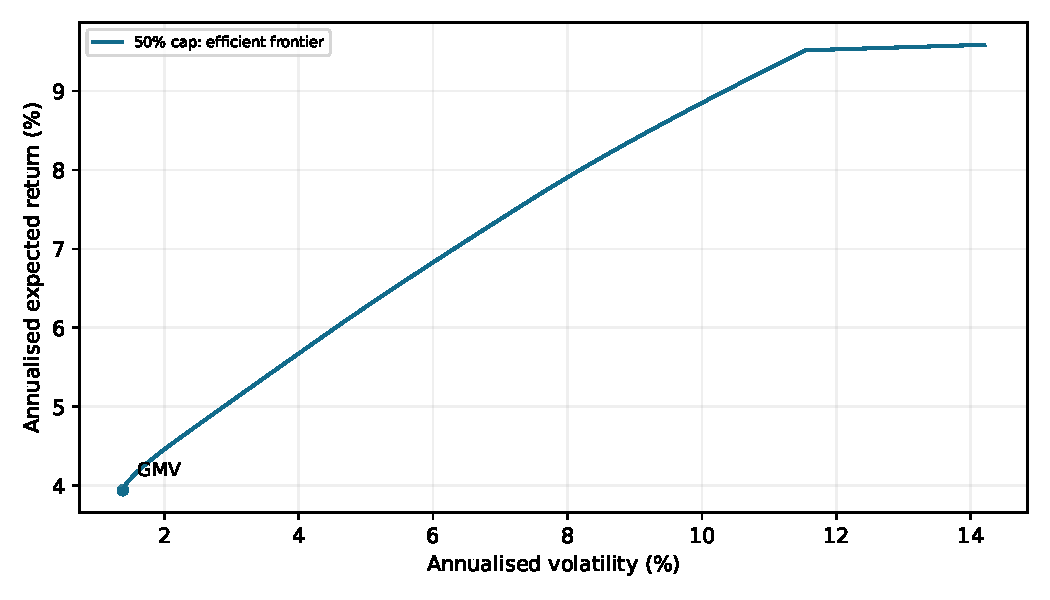
\includegraphics{../figures/Q2_baseline_frontier.pdf}
\caption{Figure 1. Full-sample efficient frontier for the adopted
long-only, 50\%-capped model. The marked GMV endpoint has expected
return 3.940\% and volatility 1.383\%.}
\end{figure}

Requirements below the GMV mean produce the same GMV portfolio;
requirements above the maximum are infeasible. The figure shows the
efficient branch, not the dominated lower-return branch.

\newpage

\hypertarget{comparison-with-alternative-constraints}{%
\subsubsection{Comparison with alternative
constraints}\label{comparison-with-alternative-constraints}}

At the same 8\% expected-return requirement, annualised volatility is:

\begin{longtable}[]{@{}lrrrr@{}}
\toprule\noalign{}
Estimation period & Uncapped & 50\% cap & 40\% cap & 30\% cap \\
\midrule\noalign{}
\endhead
\bottomrule\noalign{}
\endlastfoot
Full sample & 8.161\% & 8.186\% & 8.316\% & 8.555\% \\
Recent 10 years & 6.538\% & 6.638\% & 6.707\% & 6.882\% \\
Recent 5 years & 5.402\% & 6.014\% & 6.266\% & 6.566\% \\
\end{longtable}

Compared with the uncapped portfolio, the 50\%, 40\% and 30\% caps
produce higher fitted volatility, with the increase becoming larger as
the cap becomes more restrictive. We accept the increase under the 50\%
cap in exchange for limiting capital concentration in individual
indices. This spreads capital across at least two indices, although it
does not ensure that risk is evenly distributed.

The 50\% cap increases volatility relative to the uncapped benchmark by
approximately \textbf{0.024, 0.100 and 0.612 percentage points},
respectively. Its cost is small in the full sample but larger over five
years. Tighter caps reduce the feasible set further and cannot lower
minimum variance at a common feasible requirement.

We accept this efficiency cost to enforce the stated concentration
policy. We do not claim that 50\% is economically optimal or that the
capped portfolio must outperform the benchmark.

To examine short selling separately, we compare uncapped long-only and
unrestricted signed-weight portfolios at an 8\% requirement:

\begin{longtable}[]{@{}
  >{\raggedright\arraybackslash}p{(\columnwidth - 6\tabcolsep) * \real{0.2000}}
  >{\raggedleft\arraybackslash}p{(\columnwidth - 6\tabcolsep) * \real{0.2667}}
  >{\raggedleft\arraybackslash}p{(\columnwidth - 6\tabcolsep) * \real{0.2667}}
  >{\raggedleft\arraybackslash}p{(\columnwidth - 6\tabcolsep) * \real{0.2667}}@{}}
\toprule\noalign{}
\begin{minipage}[b]{\linewidth}\raggedright
Estimation period
\end{minipage} & \begin{minipage}[b]{\linewidth}\raggedleft
Uncapped long-only volatility
\end{minipage} & \begin{minipage}[b]{\linewidth}\raggedleft
Unrestricted volatility
\end{minipage} & \begin{minipage}[b]{\linewidth}\raggedleft
Gross exposure
\end{minipage} \\
\midrule\noalign{}
\endhead
\bottomrule\noalign{}
\endlastfoot
Full sample & 8.161\% & 6.265\% & 275.71\% \\
Recent 10 years & 6.538\% & 4.466\% & 350.12\% \\
Recent 5 years & 5.402\% & 2.331\% & 310.62\% \\
\end{longtable}

The unrestricted portfolios have no gross-exposure limit and omit
borrowing and financing costs. Their lower fitted volatility comes with
large offsetting positions.

\begin{figure}[H]
\centering
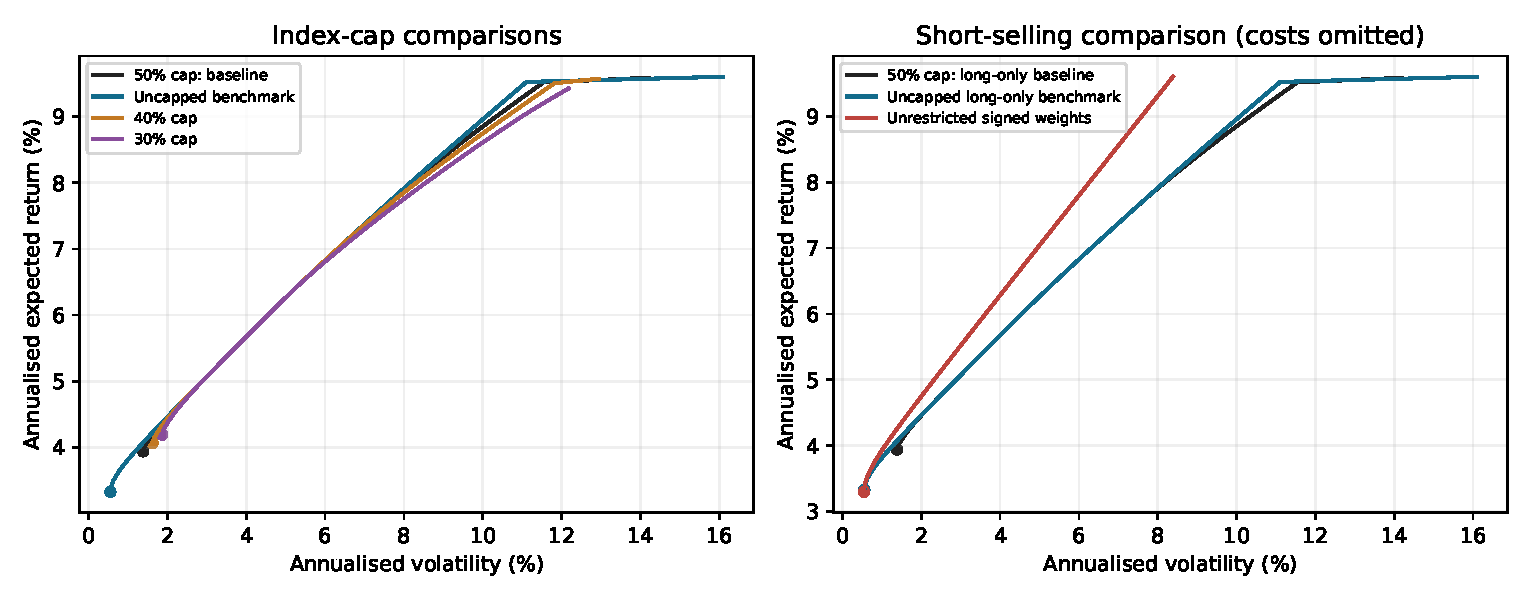
\includegraphics{../figures/Q2a_alternative_frontiers.pdf}
\caption{Figure 2. Full-sample comparisons of index caps and
short-selling assumptions. The uncapped long-only curve separates the
effect of the cap from the effect of permitting signed weights.}
\end{figure}

\newpage

\hypertarget{q2b-global-minimum-variance-portfolio}{%
\subsection{Q2(b): Global minimum-variance
portfolio}\label{q2b-global-minimum-variance-portfolio}}

\hypertarget{optimisation-and-allocation}{%
\subsubsection{Optimisation and
allocation}\label{optimisation-and-allocation}}

The GMV portfolio solves:

\[
\min_w\;w^\top Cw
\quad\text{subject to}\quad
\mathbf1^\top w=1,\quad0\leq w_i\leq0.50.
\]

There is no expected-return requirement. With positive-definite C and
linear constraints, the problem has a unique optimal weight vector. The
full-sample result is:

\begin{longtable}[]{@{}lr@{}}
\toprule\noalign{}
Index & GMV weight \\
\midrule\noalign{}
\endhead
\bottomrule\noalign{}
\endlastfoot
ASA52 & 0.0000\% \\
NDDLWI & 0.0000\% \\
NDLEEGF & 0.0000\% \\
RDAU & 0.0000\% \\
FDCIISAH & 0.0000\% \\
HEDGNAV & 16.7665\% \\
BACM0 & 15.4379\% \\
H03432AU & 17.7956\% \\
BAUBIL & 50.0000\% \\
\end{longtable}

\textbf{Annualised expected return: 3.940\%.}

\textbf{Annualised volatility: 1.383\%.}

Weights sum to 100\% before rounding. Displayed zero weights are zero
within numerical precision.

\hypertarget{interpretation}{%
\subsubsection{Interpretation}\label{interpretation}}

BAUBIL reaches its 50\% limit. The remaining allocation is split between
HEDGNAV, BACM0 and H03432AU to minimise joint portfolio variance. The
model does not require every index to be held.

Compared with uncapped GMV, the cap reduces the largest allocation from
approximately 98.28\% to 50\%, while volatility rises from 0.554\% to
1.383\%. Expected return also changes from 3.329\% to 3.940\%.

GMV minimises estimated risk. It does not maximise return or identify a
portfolio suitable for every investor. The growth/defensive and
risk-aversion objectives in later questions address different investment
needs.

The capped GMV results under alternative estimates are:

\begin{longtable}[]{@{}lrr@{}}
\toprule\noalign{}
Estimation period & GMV expected return & GMV volatility \\
\midrule\noalign{}
\endhead
\bottomrule\noalign{}
\endlastfoot
Full sample & 3.940\% & 1.383\% \\
Recent 10 years & 2.647\% & 1.574\% \\
Recent 5 years & 3.686\% & 1.718\% \\
\end{longtable}

\newpage

\hypertarget{q2c-minimum-variance-for-target-returns}{%
\subsection{Q2(c): Minimum variance for target
returns}\label{q2c-minimum-variance-for-target-returns}}

\hypertarget{problem-and-target-range}{%
\subsubsection{Problem and target
range}\label{problem-and-target-range}}

We solve the same constrained problem as Q2(a), retaining the inequality
\(m^\top w\) \(\geq\) \(\mu\). The full-sample efficient interval is
3.9403\% to 9.5866\%. In addition to the 81-point frontier, we report
requirements from 3\% to 9.5\% to show behaviour below GMV, intermediate
trade-offs and a high-return allocation near the maximum.

The maximum is attained by allocating 50\% to NDLEEGF and 50\% to
NDDLWI, the two highest estimated means. Requirements above 9.5866\% are
infeasible under the full-sample estimates and 50\% cap.

\hypertarget{full-sample-results}{%
\subsubsection{Full-sample results}\label{full-sample-results}}

\begin{longtable}[]{@{}
  >{\raggedright\arraybackslash}p{(\columnwidth - 6\tabcolsep) * \real{0.2000}}
  >{\raggedleft\arraybackslash}p{(\columnwidth - 6\tabcolsep) * \real{0.2667}}
  >{\raggedleft\arraybackslash}p{(\columnwidth - 6\tabcolsep) * \real{0.2667}}
  >{\raggedleft\arraybackslash}p{(\columnwidth - 6\tabcolsep) * \real{0.2667}}@{}}
\toprule\noalign{}
\begin{minipage}[b]{\linewidth}\raggedright
Return requirement
\end{minipage} & \begin{minipage}[b]{\linewidth}\raggedleft
Achieved expected return
\end{minipage} & \begin{minipage}[b]{\linewidth}\raggedleft
Volatility
\end{minipage} & \begin{minipage}[b]{\linewidth}\raggedleft
Largest weight
\end{minipage} \\
\midrule\noalign{}
\endhead
\bottomrule\noalign{}
\endlastfoot
3.00\% & 3.940\% & 1.383\% & 50.00\% \\
4.00\% & 4.000\% & 1.413\% & 50.00\% \\
5.00\% & 5.000\% & 2.882\% & 34.55\% \\
6.00\% & 6.000\% & 4.546\% & 29.37\% \\
7.00\% & 7.000\% & 6.310\% & 39.64\% \\
8.00\% & 8.000\% & 8.186\% & 50.00\% \\
9.00\% & 9.000\% & 10.340\% & 50.00\% \\
9.50\% & 9.500\% & 11.500\% & 50.00\% \\
\end{longtable}

At a 3\% requirement, the return constraint is inactive because GMV
already earns an estimated 3.940\%. Forcing equality to 3\% would solve
a different problem. At the reported requirements above GMV's mean, the
constraint binds and achieved expected return equals the requirement
within numerical precision.

\hypertarget{selected-allocations}{%
\subsubsection{Selected allocations}\label{selected-allocations}}

\begin{longtable}[]{@{}
  >{\raggedright\arraybackslash}p{(\columnwidth - 8\tabcolsep) * \real{0.1579}}
  >{\raggedleft\arraybackslash}p{(\columnwidth - 8\tabcolsep) * \real{0.2105}}
  >{\raggedleft\arraybackslash}p{(\columnwidth - 8\tabcolsep) * \real{0.2105}}
  >{\raggedleft\arraybackslash}p{(\columnwidth - 8\tabcolsep) * \real{0.2105}}
  >{\raggedleft\arraybackslash}p{(\columnwidth - 8\tabcolsep) * \real{0.2105}}@{}}
\toprule\noalign{}
\begin{minipage}[b]{\linewidth}\raggedright
Index
\end{minipage} & \begin{minipage}[b]{\linewidth}\raggedleft
4\% requirement
\end{minipage} & \begin{minipage}[b]{\linewidth}\raggedleft
6\% requirement
\end{minipage} & \begin{minipage}[b]{\linewidth}\raggedleft
8\% requirement
\end{minipage} & \begin{minipage}[b]{\linewidth}\raggedleft
9.5\% requirement
\end{minipage} \\
\midrule\noalign{}
\endhead
\bottomrule\noalign{}
\endlastfoot
ASA52 & 0.00\% & 0.00\% & 0.00\% & 0.00\% \\
NDDLWI & 0.00\% & 0.00\% & 4.80\% & 26.54\% \\
NDLEEGF & 0.00\% & 4.83\% & 16.44\% & 22.51\% \\
RDAU & 0.00\% & 0.00\% & 0.00\% & 0.00\% \\
FDCIISAH & 0.21\% & 23.48\% & 50.00\% & 50.00\% \\
HEDGNAV & 19.90\% & 24.13\% & 0.00\% & 0.00\% \\
BACM0 & 10.60\% & 18.19\% & 9.24\% & 0.00\% \\
H03432AU & 19.28\% & 29.37\% & 19.52\% & 0.95\% \\
BAUBIL & 50.00\% & 0.00\% & 0.00\% & 0.00\% \\
\end{longtable}

At 4\%, BAUBIL reaches its 50\% cap. At 6\%, no index reaches the cap,
and the solution matches the uncapped portfolio at that requirement. At
8\% and 9.5\%, FDCIISAH reaches 50\%, so additional expected return is
obtained through other indices rather than increasing this holding
further.

Estimated volatility rises as the required return rises. Covariances
determine which combinations meet each requirement with minimum
variance, and choosing only the highest-return index would neither
respect the cap nor reproduce these efficient allocations.

\newpage

\hypertarget{q2d-sensitivity-to-parameter-estimates}{%
\subsection{Q2(d): Sensitivity to parameter
estimates}\label{q2d-sensitivity-to-parameter-estimates}}

\hypertarget{comparison-design-and-frontiers}{%
\subsubsection{Comparison design and
frontiers}\label{comparison-design-and-frontiers}}

We repeat the optimisation using the full 248-return sample, recent 120
returns and recent 60 returns from Q1. Constraints, annualisation and
solver are unchanged. Each period uses its own expected-return vector
and covariance matrix, so differences arise from parameter estimation.

\begin{figure}[H]
\centering
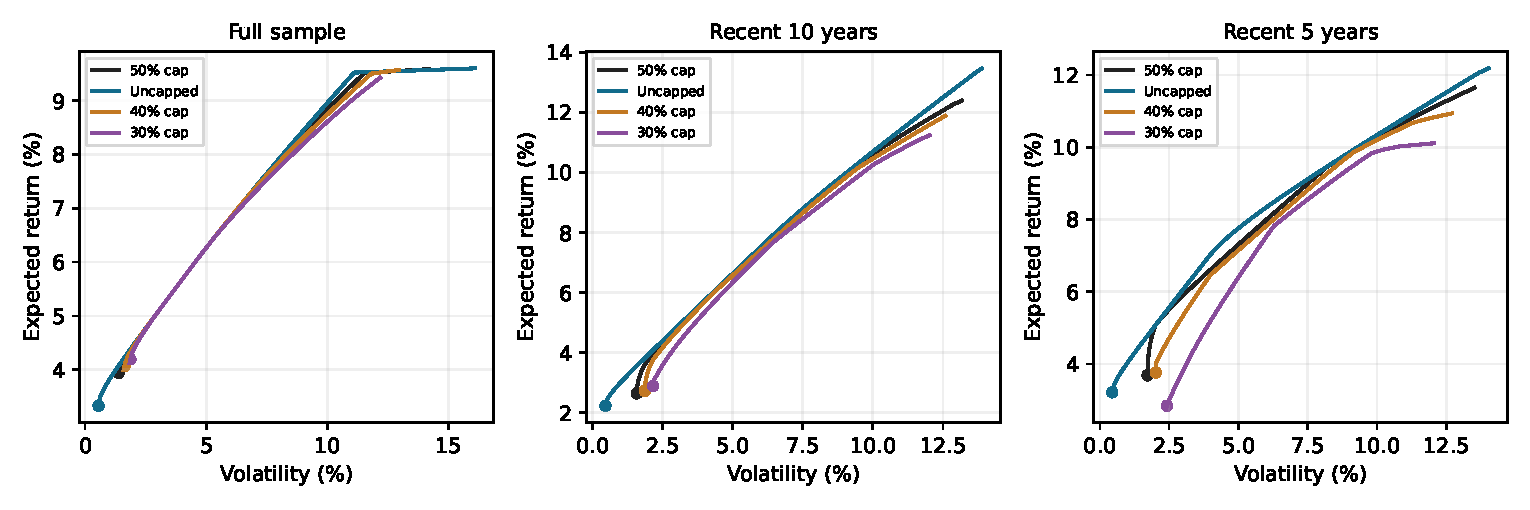
\includegraphics{../figures/Q2a_window_frontiers.pdf}
\caption{Figure 3. Efficient frontiers under the three Q1 estimation
periods. The 50\% curve is the main model in every panel; other caps and
the uncapped model remain comparisons.}
\end{figure}

For the 50\%-capped model, annualised volatility at common requirements
is:

\begin{longtable}[]{@{}
  >{\raggedright\arraybackslash}p{(\columnwidth - 8\tabcolsep) * \real{0.1579}}
  >{\raggedleft\arraybackslash}p{(\columnwidth - 8\tabcolsep) * \real{0.2105}}
  >{\raggedleft\arraybackslash}p{(\columnwidth - 8\tabcolsep) * \real{0.2105}}
  >{\raggedleft\arraybackslash}p{(\columnwidth - 8\tabcolsep) * \real{0.2105}}
  >{\raggedleft\arraybackslash}p{(\columnwidth - 8\tabcolsep) * \real{0.2105}}@{}}
\toprule\noalign{}
\begin{minipage}[b]{\linewidth}\raggedright
Estimation period
\end{minipage} & \begin{minipage}[b]{\linewidth}\raggedleft
4\% volatility
\end{minipage} & \begin{minipage}[b]{\linewidth}\raggedleft
6\% volatility
\end{minipage} & \begin{minipage}[b]{\linewidth}\raggedleft
8\% volatility
\end{minipage} & \begin{minipage}[b]{\linewidth}\raggedleft
Maximum expected return
\end{minipage} \\
\midrule\noalign{}
\endhead
\bottomrule\noalign{}
\endlastfoot
Full sample & 1.413\% & 4.546\% & 8.186\% & 9.587\% \\
Recent 10 years & 2.180\% & 4.289\% & 6.638\% & 12.392\% \\
Recent 5 years & 1.730\% & 3.138\% & 6.014\% & 11.648\% \\
\end{longtable}

At an 8\% requirement, fitted volatility changes from 8.186\% to 6.638\%
and 6.014\%. The maximum feasible expected return also changes. A lower
fitted volatility under recent estimates does not establish lower future
risk or a better estimation window, as each model evaluates portfolios
using different estimated parameters.

\newpage

\hypertarget{allocation-sensitivity}{%
\subsubsection{Allocation sensitivity}\label{allocation-sensitivity}}

The 8\% allocations are:

\begin{longtable}[]{@{}lrrr@{}}
\toprule\noalign{}
Index & Full sample & Recent ten years & Recent five years \\
\midrule\noalign{}
\endhead
\bottomrule\noalign{}
\endlastfoot
ASA52 & 0.00\% & 0.00\% & 0.00\% \\
NDDLWI & 4.80\% & 33.26\% & 28.41\% \\
NDLEEGF & 16.44\% & 0.32\% & 4.84\% \\
RDAU & 0.00\% & 0.00\% & 0.00\% \\
FDCIISAH & 50.00\% & 0.00\% & 0.00\% \\
HEDGNAV & 0.00\% & 50.00\% & 50.00\% \\
BACM0 & 9.24\% & 0.00\% & 0.00\% \\
H03432AU & 19.52\% & 0.00\% & 0.00\% \\
BAUBIL & 0.00\% & 16.42\% & 16.75\% \\
\end{longtable}

The full-sample portfolio allocates 50\% to FDCIISAH and nothing to
HEDGNAV. Both recent-window solutions allocate 50\% to HEDGNAV and
nothing to FDCIISAH. The cap prevents larger positions, but substantial
changes in the composition remain.

We measure the difference from each full-sample allocation using:

\[
D(w,\widetilde w)=\frac12\sum_i|w_i-\widetilde w_i|.
\]

For long-only portfolios, D is the fraction of capital allocated
differently, between zero and one. The following table expresses it as a
percentage. It is not realised trading turnover: these are alternative
estimates at the same end date.

\begin{longtable}[]{@{}
  >{\raggedright\arraybackslash}p{(\columnwidth - 8\tabcolsep) * \real{0.1579}}
  >{\raggedleft\arraybackslash}p{(\columnwidth - 8\tabcolsep) * \real{0.2105}}
  >{\raggedleft\arraybackslash}p{(\columnwidth - 8\tabcolsep) * \real{0.2105}}
  >{\raggedleft\arraybackslash}p{(\columnwidth - 8\tabcolsep) * \real{0.2105}}
  >{\raggedleft\arraybackslash}p{(\columnwidth - 8\tabcolsep) * \real{0.2105}}@{}}
\toprule\noalign{}
\begin{minipage}[b]{\linewidth}\raggedright
Comparison with full sample
\end{minipage} & \begin{minipage}[b]{\linewidth}\raggedleft
GMV
\end{minipage} & \begin{minipage}[b]{\linewidth}\raggedleft
4\% requirement
\end{minipage} & \begin{minipage}[b]{\linewidth}\raggedleft
6\% requirement
\end{minipage} & \begin{minipage}[b]{\linewidth}\raggedleft
8\% requirement
\end{minipage} \\
\midrule\noalign{}
\endhead
\bottomrule\noalign{}
\endlastfoot
Recent 10 years & 10.22\% & 23.59\% & 75.87\% & 94.89\% \\
Recent 5 years & 14.38\% & 15.15\% & 75.58\% & 90.36\% \\
\end{longtable}

Mean-variance portfolios are sensitive to changes in estimated returns
and covariances. The 50\% cap controls maximum allocations, but it does
not remove estimation uncertainty or make the optimal weights stable.
Later bootstrap and out-of-sample analysis are needed to assess
allocation reliability and realised outcomes.

\hypertarget{numerical-validation-and-conclusion}{%
\subsection{Numerical validation and
conclusion}\label{numerical-validation-and-conclusion}}

All 1,091 long-only solutions passed feasibility and optimality checks.
The maximum primal constraint violation was approximately
\(1.02\times10^{-14}\). Frontier variances were non-decreasing and cap
comparisons respected the expected feasible-set ordering. Signed
portfolios passed analytical feasibility and stationarity checks. The
numerical implementation uses analytic gradients and active-constraint
refinement for the convex Markowitz problem.

Our main model is fully invested, long-only and capped at 50\% per
index. It enforces a stated concentration policy while retaining the
uncapped portfolio as an efficiency benchmark. Its full-sample GMV has
expected return 3.940\% and volatility 1.383\%, with higher return
requirements increasing the fitted risk. Both the frontier and
allocations change with the estimation period.

These are fitted historical comparisons. Q1's qualifications about
currency comparability, index-return definitions and estimation
uncertainty remain relevant. The results do not establish better future
performance from imposing the cap.

For later questions, retain Q1's asset order and full-precision inputs
with weights summing to one and lying between zero and 50\%.

\end{document}
